\documentclass[../qm.tex]{subfiles}
\begin{document}
	\vfill
	\newpage
	\begin{figure}[H]
		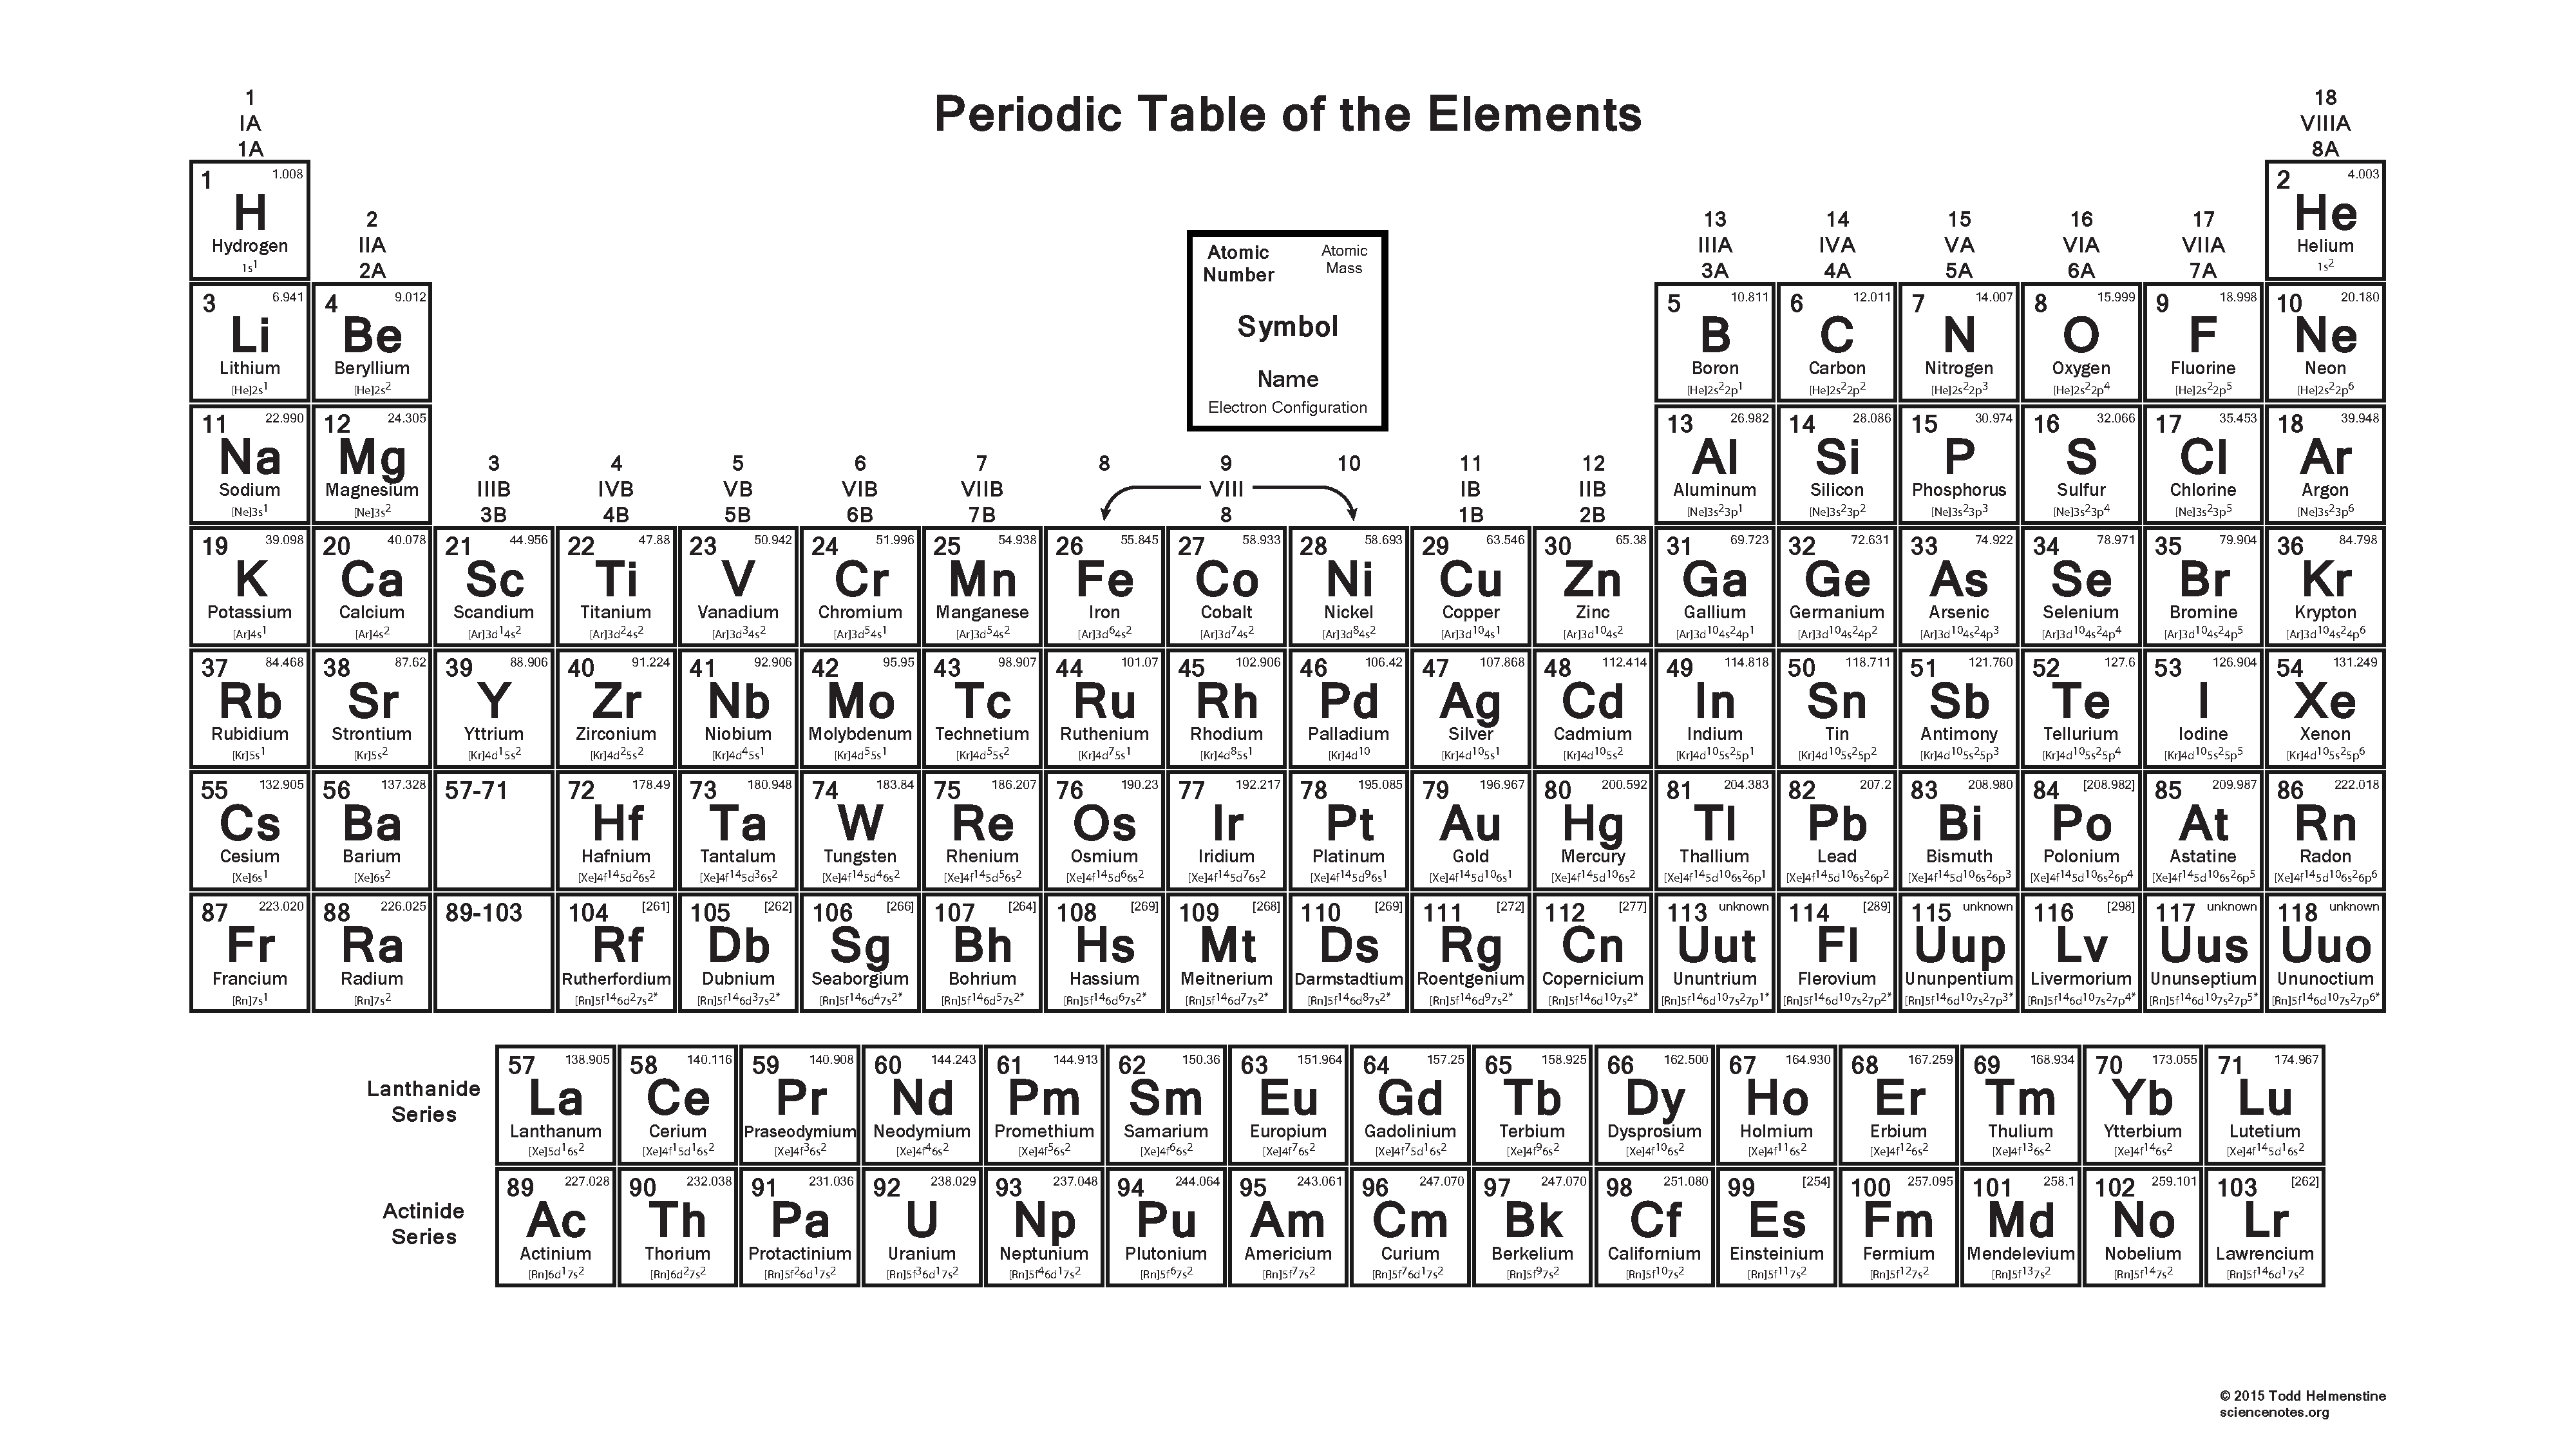
\includegraphics[angle=90, width=\linewidth]{ptwconf.pdf}
	\end{figure}
	\section{AXE Table for VSEPR Theory}
	\begin{table}[H]
	\centering
	\begin{tabular}{|c|c|c|c|c|}
		\hline
		Composition&Structure&Planar Angles&Vertical Angles&Example Compound\\\hline
		$\mathrm{AX_2}$&Linear&$180^\circ$&//&$\mathrm{BeCl_2}, \mathrm{CO_2}$\\\hline
		$\mathrm{AX_2E}$&Bent&$120^\circ\ (119^\circ)$&//&$\mathrm{NO_2^-}, \mathrm{SO_2}$\\\hline
		$\mathrm{AX_2E_2}$&Bent&$109.5^\circ\ (104.48^\circ)$&//&$\mathrm{H_2O}, \mathrm{OF_2}$\\\hline
		$\mathrm{AX_2E_3}$&Linear&$180^\circ$&//&$\mathrm{XeF_2}, \mathrm{I_3^-}$\\\hline
		$\mathrm{AX_3}$&Trigonal Planar&$120^\circ$&//&$\mathrm{BF_3}, \mathrm{SO_3}$\\\hline
		$\mathrm{AX_3E}$&Trigonal Pyramidal&$109.5^\circ\ (106.8^\circ)$&//&$\mathrm{NH_3}, \mathrm{PCl_3}$\\\hline
		$\mathrm{AX_3E_2}$&T-Shaped&$180^\circ\ (175^\circ)$&$90^\circ\ (87.5^\circ)$&$\mathrm{ClF_3}, \mathrm{BrF_3}$\\\hline
		$\mathrm{AX_4}$&Tetrahedral&$120^\circ$&$109.5^\circ$&$\mathrm{CH_4}, \mathrm{XeO_4}$\\\hline
		$\mathrm{AX_4E}$&Seesaw&$180^\circ$&$120^\circ$&$\mathrm{SF_4}$\\\hline
		$\mathrm{AX_4E_2}$&Square Pyramidal&$180^\circ$&$90^\circ$&$\mathrm{XeF_4}$\\\hline
		$\mathrm{AX_5}$&Trigonal Bipyramidal&$120^\circ$&$90^\circ$&$\mathrm{PCl_5}$\\\hline
		$\mathrm{AX_5E}$&Square Pyramidal&$90^\circ$&$90^\circ$&$\mathrm{ClF_5}, \mathrm{BrF_5}$\\\hline
		$\mathrm{AX_5E_2}$&Pentagonal Planar&$72^\circ$&$144^\circ$&$\mathrm{XeF_5^-}$\\\hline
		$\mathrm{AX_6}$&Octahedral&$90^\circ$&$90^\circ$&$\mathrm{SF_6}$\\\hline
		$\mathrm{AX_6E}$&Pentagonal Pyramidal&$72^\circ$&$90^\circ$&$\mathrm{XeOF_5^-}, \mathrm{IOF_5^{2-}}$\\\hline
		$\mathrm{AX_7}$&Pentagonal Bipyramidal&$72^\circ$&$90^\circ$&$\mathrm{IF_7}$\\\hline
		$\mathrm{AX_8}$&Square Antiprismatic&//&//&$\mathrm{IF_8^-}, \mathrm{XeF_8^{2-}}$\\\hline
		$\mathrm{AX_9}$&Tricapped Trigonal Prismatic&//&//&$\mathrm{ReH_9^{2-}}$\\\hline
	\end{tabular}
	\caption{VSEPR table for determining the molecular structure of compounds from their Lewis structure}
	\label{tab:vsepr.per}
\end{table}
\subsection{Orbital Hybridization}
In order to determine the hybridization state of molecular orbitals we have a simple algorithm that we can use, for any given atom we:
\begin{enumerate}
\item Calculate the number of atoms bound (X) to the central atom (A)
\item Count the number of lone pairs (E)
\item Sum the found values
\end{enumerate}
Therefore
\begin{equation*}
	X+E=\begin{dcases}
		2&sp\ \text{hybridization}\\
		3&sp^2\ \text{hybridization}\\
		4&sp^3\ \text{hybridization}
	\end{dcases}
\end{equation*}
There is an exception for atoms with lone pairs close to pi bonds, in fact lone pairs adjacent to pi bonds tend to stay in unhybridized p orbitals, and it's most common in nitrogen and oxygen. This can is explained thanks to the fact that this \emph{de-hybridization} can be explained via orbital overlap. A p orbital instead of a hybridized orbital leads to a ``stronger bond'' between the atoms. Always remember though that hybridization is determined by the molecular geometry and not the other way around.\\
Note that in free radicals we might find a $sp^2$ hybridization (like with carbenes and nitrenes), but due to geometrical strains the actual hybridization is way closer to a $sp^3$, and the geometry is a shallow pyramidal and not a pyramidal as we might obtain with the AXE table
\end{document}
